\chapter{Rate Limiter}\label{ch:rate-limiter}

\resilienceMechanismChapterIntro{Rate Limiter}{proactive}


\section{Introduction}\label{sec:rate-limiter-introduction}

The Rate Limiter is a proactive resilience mechanism
that aims to control the rate at which requests are made to a service or resource.
To understand this concept more thoroughly, it is important to break down the terms that compose it:

\begin{itemize}
    \item \textbf{Rate}: Refers to the frequency at which something occurs that could be bound to a time unit;
    \item \textbf{Limiter}: Refers to a mechanism that imposes a restriction or cap on the extent or quantity of something.
\end{itemize}

By combining these concepts,
a Rate Limiter
controls the frequency of requests
by setting a maximum limit on the number of requests that can be made within a given time period, as shown in Figure~\ref{fig:rate-limited-api}.
Additionally,
rate limiting can also be applied to the number of concurrent requests
that can be made simultaneously.
This helps to prevent overloading downstream services,
ensuring stability and availability of the system~\cite{microsoft-rate-limiting-pattern}.

\begin{figure}[!htb]
    \centering
    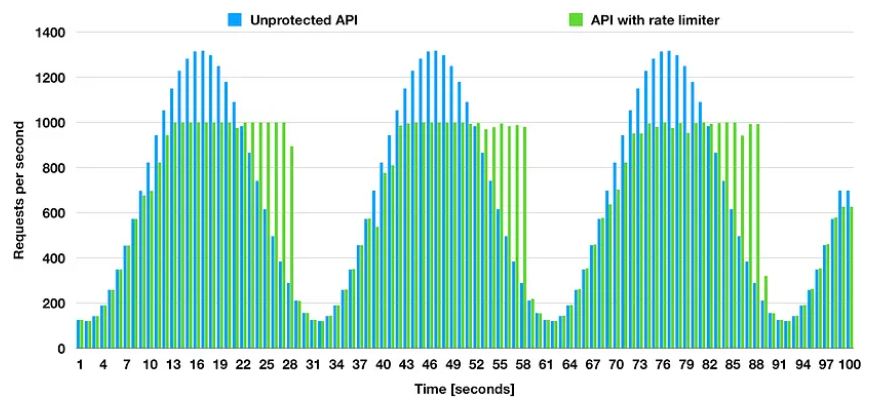
\includegraphics[width=0.8\textwidth]{../figures/06_rate_limited_api}
    \caption{API with and without Rate Limiter.
    Retrieved from~\cite{resilience4j-rate-limiter}}.
    \label{fig:rate-limited-api}
\end{figure}

Advantages of using a Rate Limiter include~\cite{solo-io-rate-limiting, kong-rate-limiting}:

\begin{itemize}
    \item \textbf{Prevent malicious activities}: Rate limiting can help protect against brute force, denial-of-service, and distributed denial-of-service (DDoS) attacks, web scraping, and other malicious activities~\cite{cloudflare-rate-limiting};
    \item \textbf{Manage Resource Utilization}: By controlling the rate of requests, rate limiting helps to manage resource utilization, prevent resource starvation, and ensure that resources are available for all users following predefined SLAs (Service Level Agreements);
    \item \textbf{Prevent Abuse}: Stops users from monopolizing resources and prevents excessive or unnecessary requests, ensuring fair resource distribution and optimal network or server performance;
    \item \textbf{Improve User Experience}: Rate limiting reduces delays and enhances the responsiveness of the service for legitimate users, improving the overall user experience;
    \item \textbf{Reduce Costs}: Helps avoid extra costs associated with overloading resources, as limiting request rates reduces the demand on resources and prevents the need for additional capacity.
\end{itemize}

\subsection{API Gateway}\label{subsec:rate-limiter-api-gateway}

An API Gateway is a server or software application that acts as an intermediary between clients and backend services or microservices.
It serves as a single entry point for API calls, managing and routing them to the appropriate services, while also providing various functionalities to enhance security, performance, and usability.

One of the key features~\cite{api-gateway} of an API Gateway's traffic management is the implementation of rate limiting and throttling policies.
These policies control the rate of incoming requests and set rules and limits to regulate traffic, preventing the overloading of backend services.

\subsection{Relation To The Throttling Mechanism}\label{subsec:rate-limiter-throttling}

Rate limiting and throttling are closely related concepts often used interchangeably,
since both mechanisms control the rate of incoming requests to protect services from being overwhelmed, but they have distinct differences.
Rate limiting refers to the process of restricting the number of requests that can be made to a service within a given time period.
Throttling, on the other hand,
specifically adjusts the flow rate based on current system load.
Is typically used to ensure that high-priority requests are served first by delaying less critical ones.

To better illustrate the difference between these two concepts, consider the following analogy:
a rate limiter is like traffic lights that control the number of cars that can pass through an intersection within a certain time frame,
whereas throttling is like adjusting the speed of cars based on traffic conditions to prevent congestion.

\subsection{Semaphore}\label{subsec:rate-limiter-semaphore}

A semaphore is a synchronization primitive that restricts the number of simultaneous accesses to a shared resource
up to a specified limit.
Key characteristics and operations of a semaphore include~\cite{java-semaphore, oracle-multithreaded-programming-guide}:

\begin{itemize}
    \item \textbf{Permits}: The semaphore keeps track of available permits.
    Each permit represents a single unit of resource access that can be granted.
    Resource access may require multiple permits, depending on the use case;
    \item \textbf{Acquire}: This operation decreases the number of available permits by a given number.
    If no permits are available, the acquiring entity is blocked (in the case of threads) or suspended (in the case of coroutines) until a permit is released;
    \item \textbf{Release}: This operation increases the number of available permits by a given number.
    Since releasing permits possibly created conditions for other entities (waiting to acquire permits) to proceed, then the semaphore notifies them.
\end{itemize}

There are two main types of semaphores:
\begin{itemize}
    \item \textbf{Binary Semaphore}:
    This type has only two states: available (1 permit) and unavailable (0 permits).
    In literature, it is also misconceptionally known as a mutex (mutual exclusion lock),
    but differs in ownership rights.
    An acquired mutex can only be released by the entity that acquired it, while a semaphore can be signalled by any other entity.
    \item \textbf{Counting Semaphore}: This type can have a count greater than one, allowing multiple entities to acquire permits up to a specified limit.
    It is used for managing access to a resource pool.
\end{itemize}

In the context of rate limiting, a semaphore can be used to control the rate of incoming requests by granting or denying access based on the availability of permits.

\subsection{Rate Limiting Algorithms}\label{subsec:rate-limiter-algorithms}

There are several algorithms that can be used to implement rate limiting, each with benefits and drawbacks to consider.
Therefore, the choice depends on the specific requirements of the system and the challenges it faces
(i.e., implementation on a single server or distributed system, handling bursty traffic, etc.)
~\cite{medium-rate-limiting-algorithms,nordic-apis-rate-limiting-algorithms}:

\subsubsection{Token Bucket}\label{subsubsec:token-bucket-algorithm}

This algorithm is used in packet-switched and telecommunications networks
to check data transmissions against defined limits on bandwidth and burstiness
(a measure of unevenness or variations in traffic flow).
The token bucket algorithm is based on the concept of a bucket that holds tokens,
where each token represents a unit of data or a permit to transmit data.
The key features of the token bucket algorithm include:

\begin{itemize}
    \item Has a fixed capacity (maximum number of tokens it can hold) and a refill rate (tokens added per unit of time);
    \item Tokens are added to the bucket at a constant rate, up to the maximum capacity;
    \item When a packet arrives, it must acquire a token from the bucket to proceed;
    \item If no tokens are available, the packet is considered non-conformant and may be dropped or delayed.
\end{itemize}

Provides a variable request rate and is suitable for handling bursts of requests,
as long as the bucket has enough tokens to accommodate them.
This algorithm can be implemented by a semaphore with no release operation, as the permits are automatically refilled at a constant rate.

\subsubsection{Leaky Bucket}\label{subsubsec:leaky-bucket-algorithm}

The leaky bucket algorithm is another rate limiting algorithm used in network traffic management, and is conceptually similar to the token bucket algorithm.
This algorithm's advantage is that it smooths out bursts of requests
and processes them at an approximately constant rate (analogous to water leaking out of a bucket at a constant rate).

However,
a burst of traffic can starve more recent requests from being processed
while providing no guarantee that requests get processed in a fixed amount of time.
Additionally, if you load balance servers for fault tolerance or increased throughput, a policy must be used to coordinate and enforce the limit between them~\cite{kong-rate-limiting}.

\subsubsection{Fixed Window Counter}\label{subsubsec:fixed-window-counter-algorithm}

The fixed window counter algorithm essentially counts the number of requests made within discrete,
fixed time intervals.

The key features of the fixed window counter algorithm include:

\begin{itemize}
    \item Requests are counted within a fixed time window (e.g., 1 second, 1 minute);
    \item When a request is made, the counter is incremented;
    \item If the counter exceeds the rate limit, the request is rejected;
    \item The counter is reset at the beginning of each time window.
\end{itemize}

The fixed window counter algorithm is easy to implement but can lead to bursty traffic patterns, as requests are not evenly distributed within the time window.
For example, if the rate limit is 5 requests per minute and a user makes 5 requests at the end of the time window, they can circumvent the limit by making 5 more requests at the beginning of the next time window, effectively doubling the allowed requests as shown in Figure~\ref{fig:fixed-window-counter-problem}.

\begin{figure}[!htb]
    \centering
    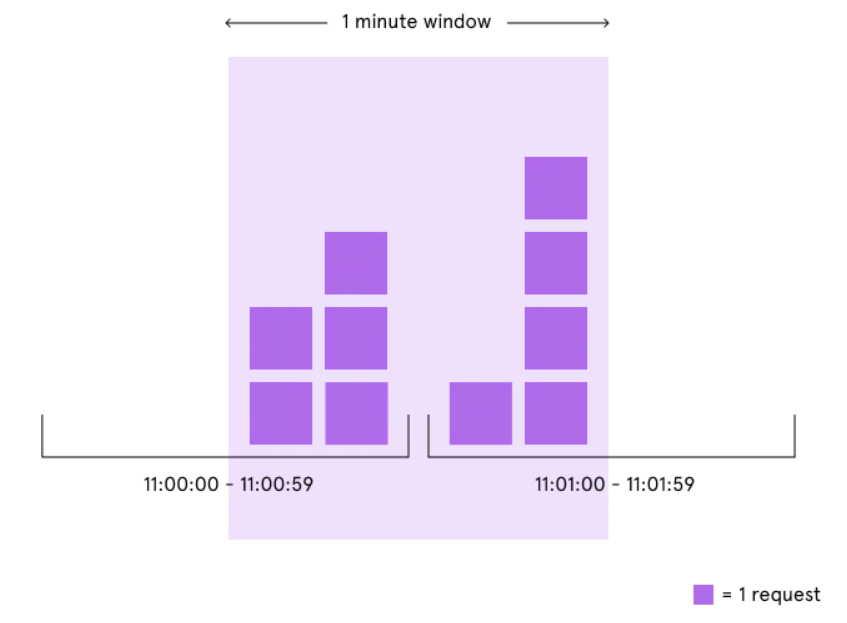
\includegraphics[width=0.5\textwidth]{../figures/06_fixed-window-counter-problem}
    \caption{Fixed Window Counter Problem.
    Retrieved from~\cite{medium-rate-limiting-algorithms}}.
    \label{fig:fixed-window-counter-problem}
\end{figure}

The fixed window counter algorithm can lead to a stampeding effect,
where previously rejected requests are retried simultaneously when the time window resets.
This effect can cause spikes in traffic and overload the system, especially when dealing with a large number of clients.
Additionally, this algorithm is behaviorally similar to the token bucket algorithm,
but the latter allows for a gradual accumulation of tokens over time never exceeding the maximum capacity
(e.g., 2 tokens per second, up to a maximum of 10 tokens), whereas the former resets the counter at the beginning of each time window.

This algorithm can be implemented using a semaphore with an automatic release operation that is triggered at the beginning of each time window.

\subsubsection{Sliding Window Log}\label{subsubsec:sliding-window-log-algorithm}

The sliding window log algorithm maintains a continuous record of requests over a rolling time period.

Key features of the sliding window log algorithm include:

\begin{itemize}
    \item Tracks requests within a continuously moving window (e.g., last 60 seconds);
    \item Maintains a log of timestamps for each request in the sliding window;
    \item Checks the log to count the number of requests in the current window whenever a new request is made;
    \itme As time progresses, the sliding window shifts, adding new requests to the log and removing old ones that fall outside the current window.
    \item Rejects the request if the sum of requests in the current window exceeds the rate limit.
\end{itemize}

Unlike the fixed window counter algorithm,
the sliding window log algorithm provides a more accurate representation of request rates over time,
and it does not suffer from the boundary conditions of fixed windows.
However, it can be memory-intensive, as it stores a timestamp for each request, and computationally expensive,
as each request requires summing up prior requests, which may not scale well in high-throughput scenarios.

\subsubsection{Sliding Window Counter}\label{subsubsec:sliding-window-counter-algorithm}

The sliding window counter algorithm essentially combines the fixed window counter and sliding window log algorithms to provide a more balanced approach to rate limiting.

Key features of the sliding window counter algorithm include:

\begin{itemize}
    \item Divides the time window into smaller fixed segments (e.g., 1-second segments within a 60-second window);
    \item Tracks the count of requests for each segment;
    \item Calculates the total number of requests in the current window by summing the counts of the relevant segments;
    \item Rejects the request if the total number of requests within the sliding window exceeds the rate limit;
    \item Continuously updates the sliding window by shifting the segments as time progresses, ensuring an accurate count for the current window.
\end{itemize}

This hybrid approach smooths out traffic bursts
by weighting the previous window’s request rate based on the current timestamp,
similar to the sliding log method
(e.g., if the current window is 25\% through, the previous window's count is weighted by 75\%).
The sliding window counter algorithm provides the flexibility to scale rate limiting with good performance,
avoiding the starvation problem of the leaky bucket and the burstiness at the boundary of fixed window implementations~\cite{kong-rate-limiting}.

\subsection{Rate Limit Exceeded}\label{subsec:rate-limiter-exceeded}

Rate limiting algorithms can be configured
to deploy different strategies for handling requests when the rate limit is exceeded
(rate-limited requests).
The most common approaches include:

\begin{itemize}
    \item \textbf{Reject}: Immediately deny the request and return an error response message (e.g., throwing an exception,
    returning an HTTP status code such as 429 - Too Many Requests), indicating that the rate limit has been reached;
    \item \textbf{Wait}: Place the request in a queue to be processed later when the rate limit allows, ensuring that the request is not lost and will eventually be handled;
    \item \textbf{Both}: Combine the previous two approaches by placing the request in a queue with a timeout.
    If the request cannot be processed within the timeout period, it is rejected.
\end{itemize}

\subsection{Types Of Rate Limiting}\label{subsec:rate-limiter-types}

Besides the algorithm-based classification, rate limiting can be implemented in various ways depending on the criteria used to limit the rate of requests.
A few common types of rate limiting include:
\begin{itemize}
    \item \textbf{Total Requests}: Limits the total number of requests to a service within a given time period.
    \item \textbf{Key-Based}: Limits requests based on specific keys, such as user ID, IP address, or API key,
    allowing different limits for different users, groups or clients.
    \item \textbf{User-Based}: Applies rate limits per user,
    ensuring that individual users cannot exceed their allocated request quota as agreed in the SLA.
\end{itemize}

\subsubsection{Available Solutions}\label{subsubsec:rate-limiter-solutions}

Following some of the state-of-the-art libraries that provide rate limiting solutions,
Resilience4j offers two distinct implementations: an atomic rate limiter and a semaphore-based rate limiter.
The atomic rate limiter uses lock-free algorithms and non-blocking operations to control the rate of requests,
while the semaphore-based rate limiter employs a lock-based semaphore and a scheduler to refill it,
blocking requests when the rate limit is exceeded.

Polly provides a thin layer over the .NET \texttt{System.Threading.RateLimiting}~\cite{microsoft-rate-limiting-dotnet} package, which includes, besides the algorithm-based, the following rate limiting implementations:
\begin{itemize}
    \item \texttt{ConcurrencyLimiter}: Limits the number of concurrent requests that can be made to a service;
    \item \texttt{PartitionedRateLimiter}: Allows rate limiting based on different keys or partitions;
    \item \texttt{ChainedPartitionedRateLimiter}:
    Chains multiple rate limiters together to provide a cascading rate limiting strategy (e.g., first check a global rate limiter, then a more specific partitioned rate limiter).
    If one rate limiter fails, all previously acquired permits are released, ensuring atomicity in rate limiting decisions.
\end{itemize}

Additionally, the package allows configuration of custom policies for handling rate limit exceedances, including queue processing strategies (e.g., newest first, oldest first) and auto-replenishment of permits.
Just as Resilience4j, Polly offers a lock-free version of the token bucket algorithm for improved performance in high-throughput scenarios.

At the time of writing, none of the mentioned libraries provide a distributed rate limiting solution,
which is a common requirement in modern architectures where services are deployed across multiple nodes.

\subsection{Distribution}\label{subsec:rate-limiter-distribution}

In a distributed system,
rate limiting can be challenging due to the need
to maintain consistency across multiple instances of the rate-limited service.
One simple way to enforce the limit is
to set up sticky sessions in the load balancer so that each consumer gets sent to exactly one node.
However, this approach has several disadvantages,
including a lack of fault tolerance and scaling problems when nodes get overloaded~\cite{kong-rate-limiting}.

A better option is to use a shared data store (e.g., a database) to store the rate limit state,
allowing all instances of the service to access and update the state in a consistent manner.
This approach has the disadvantage
of introducing additional latency due to network communication with the data store and race conditions when
multiple instances try to update the state simultaneously.

A naive approach to distributed rate limiting is to use a `get-then-set' approach,
where the rate limit state is read from the data store, incremented, and then written back.
The issue with this model is that during the read-increment-store cycle, additional requests may arrive, leading each to attempt storing an incremented counter-value, potentially resulting in an invalid (lower) counter-value.
This can enable consumers to send a high rate of requests, bypassing rate limiting controls~\cite{kong-rate-limiting}.

A few solutions arise to address these challenges:

\begin{itemize}
    \item \textbf{Locks}: Prevent concurrent access to the rate limit state by using locks to synchronize access.
    However, locks can introduce performance bottlenecks in high-concurrency scenarios;
    \item \textbf{Atomic Operations}:
    Use atomic operations provided by the data store to increment and check counters efficiently.
    Using more of the `set-then-get' approach can reduce the number of round trips to the data store;
\end{itemize}

To minimize latency introduced by using a shared data store,
rate limit checks can be performed locally in memory with an eventually consistent model as shown in Figure~\ref{fig:distributed-rate-limiting-shared}.
Each node periodically syncs with the shared store,
pushing counter-increments and retrieving updated values (to update the local cache).
\textit{\enquote{The periodic rate at which nodes converge should be configurable. Shorter sync intervals will result in less divergence of data points when spreading traffic across multiple nodes in the cluster (e.g., when sitting behind a round robin balancer). Whereas longer sync intervals put less read/write pressure on the datastore and less overhead on each node to fetch new synced values}}~\cite{kong-rate-limiting}.

\begin{figure}[!htb]
    \centering
    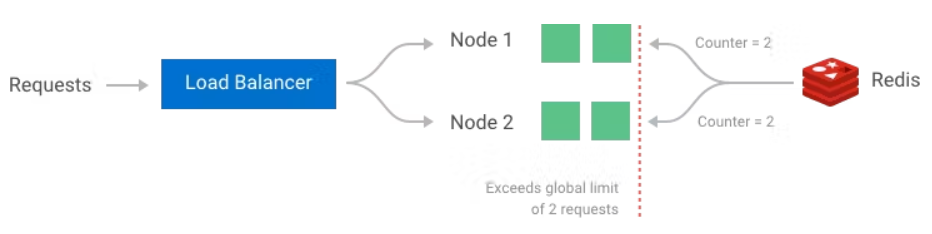
\includegraphics[width=0.8\textwidth]{../figures/06_distributed_rate_limiting}
    \caption{Distributed Rate Limiting with a Shared Data Store.
    Retrieved from~\cite{kong-rate-limiting}}.
    \label{fig:distributed-rate-limiting-shared}
\end{figure}


\section{Implementation Aspects}\label{sec:rate-limiter-implementation}

\subsection{Semaphore-Based Rate Limiter}\label{subsec:rate-limiter-semaphore-based}

The semaphore-based rate limiter is a simple yet effective way to control the rate of requests to a service.
This semaphore controls both the rate frequency and rate concurrency of requests by granting or denying access based on the availability of permits.

The implementation uses a counting semaphore based on a specified algorithm
(e.g., token bucket, fixed window counter) to apply rate limiting behaviour, namely,
the replenishment of permits as described in the respective sections.

\subsubsection{Synchronization Style}\label{subsubsec:rate-limiter-synchronization-style}

The adopted synchronization style for the semaphore-based rate limiter was the Kernel or Delegation of execution in favor of the Monitor style.

In the Monitor style of synchronization, the thread that creates or sees favorable conditions for other threads to advance to the next state, will signal those threads. It is the responsibility of those other threads to complete their own request of sorts after they exit the condition where they were waiting upon.

In the Kernel or Delegation of execution synchronization style,
the thread that creates or sees favorable conditions for other threads to advance to the next state is responsible
for completing the requests of those other threads.
In successful cases,
the threads in the dormant state that were signaled do not have
to do anything besides confirming that their request was completed and return immediately from the synchronizer.
This style of synchronization is usually associated with one or more requests that a thread wants to see completed.
These same threads will delegate the completion of the requests to another thread,
while keeping a local reference to it.
This in turn will enable the synchronizer to resume its functions without waiting for the requests to be completed.

The mentioned local reference is what
enables the thread to not lose track of the synchronizer state that it was waiting upon.
Whereas, in the monitor-style synchronization, such state could be potentially lost since the thread,
when awakened, has to recheck it which could have changed in the meantime.

\subsubsection{Algorithm Template}\label{subsubsec:rate-limiter-algorithm-template}

Initially, the semaphore-based rate limiter only supported the Fixed Window Counter algorithm indirectly.
However, the API has been redesigned to be extensible, based on the Template Method pattern,
allowing for the integration of the various rate limiting algorithms as described in the previous sections.
This new design provides callers with the flexibility to choose the algorithm that best suits their use case.

\subsubsection{Drain Operation}\label{subsubsec:rate-limiter-drain-operation}

Besides the standard acquire and release operations, the semaphore-based rate limiter also supports a drain operation.
This operation drains all available permits left in the current time window.
It is performed based on a configurable response received from the underlying rate-limited service.
This is useful for scenarios where the service needs to indicate that it is overwhelmed or needs a break,
this way pausing / delaying incoming requests effectively, allowing the service to recover.

\subsection{Available Types and Distribution}\label{subsec:rate-limiter-types-distribution}

The semaphore-based rate limiter controls the rate of requests to a service
using a counting semaphore to manage permits.
This approach ensures that the rate and concurrency of requests are limited according to the availability of permits,
which are managed based on the specified rate limiting algorithm (e.g., token bucket, fixed window counter),
as described in the previous sections.

In addition to the basic rate limiting mechanism, it was designed, through composition, a keyed rate limiter.
The keyed rate limiter provides a fine-grained approach to rate limiting
by allowing different rate limits to be set for different keys
(e.g., user ID, IP address, API key).
In this way, the rate of requests can be controlled separately for each key, as the state is maintained
independently for each key.
This approach is useful for scenarios
where different clients or users have different rate limits based on their usage patterns or SLAs,
and the abuse of one client does not affect the rate limit of another.

Both the basic and keyed rate limiters are designed to support distributed environments.
In these settings, the state (e.g., available permits, timestamps) can be stored in a shared data store,
which must be implemented manually.
By default, the rate limiter uses an in-memory data store to manage the state.
However,
the API is designed to allow replacement with a distributed data store
(e.g., Redis, Cassandra) to ensure consistency across multiple instances of the rate-limited service.

TODO(drawing for keyed rate limiter)

\subsection{Disposable Resource}\label{subsec:rate-limiter-disposable-resource}

In certain implementations, the rate limiter may need to manage resources that require proper cleanup when they are no longer needed.
For example, if the rate limiter maintains open connections to a database or a distributed data store
for storing the state, it is crucial to release these resources gracefully to prevent resource leaks and ensure system stability.

To address this, the rate limiter implements a disposable pattern,
providing a mechanism to close or dispose of any open resources~\cite{microsoft-dispose-pattern}. This mechanism should be called when the rate limiter is no longer needed, such as during application shutdown or when the rate limiter is being replaced or reconfigured.

\subsection{Retry After Policy}\label{subsec:rate-limiter-retry-after-policy}

In some use cases, when a request is rate-limited, it is useful to inform the client about when they should retry the request~\cite{mdn-retry-after}.
For instance, in the Fixed Window Counter algorithm,
the optimal time for the client to retry is at the beginning of the next time window
(i.e., the retry duration is algorithm-specific).

With this information,
an (outer) retry mechanism can be configured in the pipeline before the
(inner) rate limiter to retry the request after the recommended duration.

TODO (make drawings for the Fixed Window Counter and Sliding Window Counter algorithms retry after duration)

\subsection{Dynamic Configuration}\label{subsec:rate-limiter-dynamic-configuration}

Modern rate limiters often need to adapt to changing conditions and requirements dynamically.
Dynamic configuration allows modifying the rate limiter's behavior at runtime.

A challenge arises when changing the rate limiter's configuration dynamically: such changes can only take effect in
the next replenishment period.
If applied immediately, the retry-after policy, for example, would be inconsistent with the new configuration,
causing previously rate-limited requests to retry based on outdated information.

To address this challenge, the rate limiter provides mechanisms to update the configuration dynamically, including the
replenishment period and the total number of permits.

Additionally, it's worth noting that in distributed environments that use an eventually consistent model for rate limiting,
it can be challenging to ensure that configuration changes are propagated consistently across all nodes.

\subsection{Event Emission}\label{subsec:rate-limiter-event-emission}

The rate limiter emits events to notify listeners when a request to a rate-limited service:

\begin{itemize}
    \item Has succeeded to be processed;
    \item Has been rate-limited.
    Two different event types can be emitted in this case based on if the request was immediately rejected or queued.
\end{itemize}


\section{Configuration}\label{sec:rate-limiter-configuration}

\resilienceMechanismConfigIntroToTable{Rate Limiter}~\ref{tab:ratelimiter-config-builder}.

\begin{table}[!htb]
    \centering
    \caption{Configuration Properties for \texttt{RateLimiterConfigBuilder}}
    \label{tab:ratelimiter-config-builder}
    \vspace{0.3cm}
    \begin{tabular}{|p{5cm}|p{5cm}|p{6cm}|}
        \hline
        \textbf{Config Property} & \textbf{Default Value/Behaviour}                                                   & \textbf{Description}                               \\ \hline
        \texttt{algorithm}       & \texttt{FixedWindowCounter[ totalPermits=1000, replenishPeriod=1m, queueLength=0]} & The rate limiting algorithm and its configuration.                                                                                                         \\ \hline
        \texttt{baseTimeoutDuration} & \texttt{1s} & The default duration a request will be placed in the queue
        if rate-limited.
        After this duration, the request will be rejected. \\ \hline
        \texttt{onRejected} & \texttt{Rethrow throwable
        if any} & The exception handler that will be called when a request is rejected by the rate limiter. \\ \hline
    \end{tabular}
\end{table}

\resilienceMechanismDefaultConfig


\section{Ktor Integration}\label{sec:rate-limiter-ktor-integration}

TODO()

\subsection{Plugin Implementation}\label{subsec:rate-limiter-plugin}

TODO()

\subsection{Configuration}\label{subsec:rate-limiter-configuration}

TODO()
